\documentclass{article}
\usepackage{amsmath}
\usepackage{algpseudocode}
\usepackage{tikz}
\title{Bezier Shape Functions}
\author{Dan Zaide}
\begin{document}
\maketitle

\section{Bezier Curves}
The Bezier curve, $\mathbf{B}(t)$ of order $P$ is polynomial defined by the set of control points $\mathbf{C}_i$ for $i = 0,\ldots,P$ as 
\[
\mathbf{B}(t) = \displaystyle \sum_{i=0}^P {P \choose i}t^i(1-t)^{P-i}\mathbf{C}_i
\]
where ${P \choose i}= \frac{P!}{i!(P-i)!}$ is the binomial coefficient and $ t \in [0,1]$. The derivatives are
\[
\frac{\mathrm{d} \mathbf{B}(t)}{\mathrm{d} t} = \displaystyle \sum_{i=0}^P {P \choose i}(i-Pt)t^{i-1}(1-t)^{P-i-1}\mathbf{C}_i
\]
and
\[
\frac{\mathrm{d}^2 \mathbf{B}(t)}{\mathrm{d} t^2} = \displaystyle \sum_{i=0}^P {P \choose i}((P-1)Pt^2-2i(P-1)t+i(i-1))t^{i-2}(1-t)^{P-i-2}\mathbf{C}_i
\]
where
\[\left.\frac{\mathrm{d}^2 \mathbf{B}(t)}{\mathrm{d} t^2}\right|_t=0 = P(P-1)(\mathbf{C}_0-2\mathbf{C}_1+\mathbf{C}_2)\]
In the current implementation in \texttt{BezierShape} in \texttt{apfBezier.cc}, the edge shape functions are ordered with the vertices first, as $v_0,v_1,e_0,\ldots,e_{p-1}$, which is not geometric order.
\subsection{Interpolating Bezier Curves}
To fit a bezier curve to a known geometry, interpolating points, $\mathbf{P}_j = \mathbf{P}(t_j)$, are first needed at $t_0,\ldots, t_{P+1}$ before the control points can be solved for. This requires solving

\[
\mathbf{B}(t_j) = \displaystyle \sum_{i=0}^P {P \choose i}t_j^i(1-t_j)^{P-i}\mathbf{C}_i = \mathbf{P}_i
\]
at each interpolating point, resulting in a linear system of equations for $\mathbf{C}_i$. The following matlab code solves for these coefficients, which each row of $\mathbf{A}^{-1}$ corresponding to coefficients for the interpolating points. The first six orders are implemented in \texttt{convertEdgeLocations2D} and \texttt{convertEdgeLocations3D}.

% \begin{verbatim}
% switch (n)
%     case 2
%         t = [-1,0,1];
%     case 3
%         %         t = [-1,-0.4306648,0.4306648,1];
%         t = [0,0.2748043,0.7251957,1];
%     case 4
%         %         t = [-1,-0.6546,0.0,0.6546,1];
%         t = [0,0.1693976,0.5,0.8306024,1];
%     case 5
%         %         t = [-1,-0.7485748,-0.2765187,0.2765187,0.7485748,1];
%         t = [0, 0.1257126, 0.36174065, 0.63825935,0.8742874,1];
%     case 6
%         %         t = [-1,-0.8161268,-0.4568660,0.0, 0.4568660,0.8161268,1];
%         t = [   0, 0.0919366, 0.271567, 0.5, 0.728433, 0.9080634,1];
% end
% t(end) = [];
% t = [t(1),1,t(2:end)];
% % t = (t+1)/2;

% A = zeros(n,n);
% for i=0:n
%     bi = factorial(n)/factorial(n-i)/factorial(i);
%     for j=0:n
%         A(j+1,i+1) = bi*t(j+1)^i*(1-t(j+1))^(n-i);
%     end
% end
% Ai = inv(A);

% for i = 1:n+1
%     fprintf('{')
%     for j = 1:n+1
%         fprintf(num2str(Ai(i,j),9))
%         if (j ~= n+1)
%             fprintf(',')
%         end
%     end
%     fprintf('},\n')
    
% end
% \end{verbatim}
Several choices of $t_j$ exist. Using equally spaced $t$'s works fairly well, but closer to optimal points are in \textit{Approximate optimal points for polynomial interpolation of real functions in an interval and in a triangle}, Chen and Babuska, 1995.
\section{Bezier Triangles}
The Bezier triangle is similar, with each edge its own Bezier curve. For an order $P$ triangle, there are $(P+1)(P+2)/2$ control points, with $(P-1)(P-2)/2$ points on the interior. Using barycentric coordinates $u,v,w = 1-u-v$ we can define the Bezier triangle as 
\[
\mathbf{B}(u,v) = \displaystyle\sum_{i,j,k\geq 0}^{i+j+k=P} \frac{P!}{i!j!k!}u^iv^jw^k \alpha^i\beta^j\gamma^k 
\]
where $\alpha^i\beta^j\gamma^k$ correspond to the control points. This is implemented in a single array with size $(P+1)(P+2)/2$. The summation is then rewritten as
\[
\mathbf{B}(u,v) = \displaystyle\sum_{i=0}^P \sum_{j=0}^{P-i}\frac{P!}{i!j!(P-i-j)!}u^iv^j(1-u-v)^{P-i-j}\mathbf{P}_\ell, \quad \ell = (P+1)j+i-j(j-1)/2
\]
which is equivalent to a $[P\times P]$ triangular matrix with entries at $(i,j)$ and $k$ as follows, shown for $P = 3$
\begin{verbatim}
 j 0 1 2 3
ik________
0 |3 2 1 0
1 |2 1 0   
2 |1 0 
3 |0 
\end{verbatim}
The array indices are $\ell = (P+1)j+i-j(j-1)/2$ and are columnwise,
\begin{verbatim}
 j 0 1 2 3
i ________ 
0 |0 4 7 9
1 |1 5 8   
2 |2 6 
3 |3 
\end{verbatim}
In each case, the control points attached to each entity are ordered counter clockwise as
\begin{verbatim}
 j 0   1   2   3
i _______________ 
0 |v2  e10 e10 v1
1 |e20 f0  e01   
2 |e21 e00 
3 |v0 
\end{verbatim}
In the actual implementation, vertices are the first three points, edges are the next $3(P-1)$ and faces are the rest. So our list of points is actually $v_0,v_1,v_2,e_{0,0},\ldots,e_{0,P-1},e_{1,0},\ldots,e_{1,P-1},e_{2,0},\ldots,e_{2,P-1},f_0,\ldots,f_{(P-1)(P-2)/2}$. This is much harder to write in index form, so in the implementation. this ordering is stored as a map, and called upon when getting values or local gradients. The gradients are easily computed as 
\begin{eqnarray*}
\frac{\partial \mathbf{B}(u,v)}{\partial u} &=& \displaystyle\sum_{i=0}^P \sum_{j=0}^{P-i}\frac{P!}{i!j!(P-i-j)!}((1-v)i-(P-j)u)u^{i-1}v^j(1-u-v)^{P-i-j-1}\mathbf{P}_\ell \\
\frac{\partial \mathbf{B}(u,v)}{\partial v} &=& \displaystyle\sum_{i=0}^P \sum_{j=0}^{P-i}\frac{P!}{i!j!(P-i-j)!}((1-u)j-(P-i)v)u^{i}v^{j-1}(1-u-v)^{P-i-j-1}\mathbf{P}_\ell
\end{eqnarray*}
\subsection{Triangular Blending}
For faces not on a boundary, triangular blending of shape functions is needed. This occurs for all 2D triangles and 3D interior triangles with an edge or more on the boundary. For a given entity on the mesh, we have a coordinate field such that 
\[ \mathbf{x}(\xi) = \sum_{i=0}^N w_i(\xi) \cdot \mathbf{x}_i \]
for an entity with $N$ total nodes, where $\xi = (u,v,w) = (\xi_0,\xi_1,\xi_2)$ and $\xi_2 = 1-\xi_0-\xi_1$. To implement the blending in our framework, we have 
\[\mathbf{x}_{face}(\xi) = \sum_{i=0}^{3}||\xi_{e_i}||\sum_{j=0}^{N_{edge}}w_{e_i,j}(\xi_{e_i})\cdot\mathbf{x}_{e_i,j}- \sum_{i=0}^{3}\xi_i\mathbf{x}_{v_i}\]
Where the edge parameters are
\begin{eqnarray*} 
\xi_{e_0} & = & \frac{\xi_1}{\xi_0+\xi_1},\quad ||\xi_{e_0}|| = \xi_0+\xi_1 \\
\xi_{e_1} & = & \frac{\xi_2}{\xi_1+\xi_2},\quad ||\xi_{e_1}|| = \xi_1+\xi_2 \\
\xi_{e_2} & = & \frac{\xi_0}{\xi_2+\xi_0},\quad ||\xi_{e_2}|| = \xi_2+\xi_0 
\end{eqnarray*}
Based on the canonical ordering of edges and faces. When any of $||\xi_{e_i}|| = 0$, we are either on a vertex opposite that edge, or on a different edge, and do not consider the contribution of those edges.

The goal is then to find face weights such that \[\mathbf{x}_{face}(\xi) = \sum_{i=0}^{N_{face}} w_i(\xi) \cdot \mathbf{x}_i = \sum_{i=0}^{3}||\xi_{e_i}||\sum_{j=0}^{N_{edge}}w_{e_i,j}(\xi_{e_i})\cdot\mathbf{x}_{e_i,j}- \sum_{i=0}^{3}\xi_i\mathbf{x}_{v_i} \] 
This is a bookkeeping exercise, since every $x_{e_i,j}$ corresponds to a point on the face, in $x_i$. Consider the third-order triangle, and its edges.
\begin{figure}
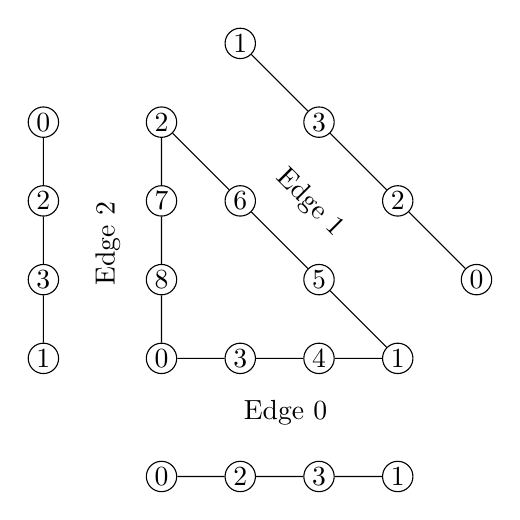
\begin{tikzpicture}[scale=1]
\tikzstyle{every node}=[circle, draw, fill=white,
                        inner sep=1pt, minimum width=4pt]
\path (0,0) node (p0) {$0$}
(1,0) node [label={[label distance=0.1cm]-60:Edge 0}] (p1) {$3$}
(2,0) node (p2) {$4$}
(3,0) node (p3) {$1$}
(2,1) node (p4) {$5$}
(1,2) node [label={[label distance=0.1cm,rotate=-45]10:Edge 1}] (p5) {$6$}
(0,3) node (p6) {$2$}
(0,2) node [label={[label distance=0.2cm,rotate=90]-200:Edge 2}] (p7) {$7$}
(0,1) node (p8) {$8$}
% (1,1) node (p9) {$9$}
(0,-1.5) node (p10) {$0$}
(1,-1.5) node (p11) {$2$}
(2,-1.5) node (p12) {$3$}
(3,-1.5) node (p13) {$1$}
(-1.5,0) node (p14) {$1$}
(-1.5,1) node (p15) {$3$}
(-1.5,2) node (p16) {$2$}
(-1.5,3) node (p17) {$0$}
(1,4) node (p18) {$1$}
(2,3) node (p19) {$3$}
(3,2) node (p20) {$2$}
(4,1) node (p21) {$0$};
\draw (p0) -- (p1)
(p1) -- (p2)
(p2) -- (p3)
(p3) -- (p4)
(p4) -- (p5)
(p5) -- (p6)
(p6) -- (p7)
(p7) -- (p8)
(p8) -- (p0)
(p10) -- (p11)
(p11) -- (p12)
(p12) -- (p13)
(p14) -- (p15)
(p15) -- (p16)
(p16) -- (p17)
(p18) -- (p19)
(p19) -- (p20)
(p20) -- (p21);
\end{tikzpicture}
\end{figure}
The face has 9 nodes associated with it, ordered as shown. The weights are then 
\begin{eqnarray*}
w_0 & = & ||\xi_{e_0}||w_{e_0,0}(\xi_{e_0}) + ||\xi_{e_2}||w_{e_2,1}(\xi_{e_2}) - \xi_0 \\
w_1 & = & ||\xi_{e_0}||w_{e_0,1}(\xi_{e_0}) + ||\xi_{e_1}||w_{e_1,0}(\xi_{e_1}) - \xi_1 \\
w_2 & = & ||\xi_{e_2}||w_{e_2,0}(\xi_{e_2}) + ||\xi_{e_1}||w_{e_1,1}(\xi_{e_1}) - \xi_2 \\
w_3 & = & ||\xi_{e_0}||w_{e_0,2}(\xi_{e_0}) \\
w_4 & = & ||\xi_{e_0}||w_{e_0,3}(\xi_{e_0}) \\
w_5 & = & ||\xi_{e_1}||w_{e_1,2}(\xi_{e_1}) \\
w_6 & = & ||\xi_{e_1}||w_{e_1,3}(\xi_{e_1}) \\
w_7 & = & ||\xi_{e_2}||w_{e_2,2}(\xi_{e_2}) \\
w_8 & = & ||\xi_{e_2}||w_{e_2,3}(\xi_{e_2}) 

\end{eqnarray*}
This is implemented in a much more generic form, using the triangle-edge ordering in \texttt{apfMesh.cc}. The local gradients are then
\begin{eqnarray*}\frac{\partial \mathbf{x}(\xi)}{\partial \xi_k}& = & \sum_{i=0}^N \frac{\partial w_i(\xi)}{\partial \xi_k} \cdot \mathbf{x}_i \\
\frac{\partial \mathbf{x}(\xi)}{\partial \xi_k}& = & \frac{\partial}{\partial \xi_k}\left[\sum_{i=0}^{3}||\xi_{e_i}||\sum_{j=0}^{N_{edge}}w_{e_i,j}(\xi_{e_i})\cdot\mathbf{x}_{e_i,j}- \sum_{i=0}^{3}\xi_i\mathbf{x}_{v_i}\right] \\ & & 
\sum_{i=0}^{3}\frac{\partial}{\partial \xi_k}\left[||\xi_{e_i}||\sum_{j=0}^{N_{edge}}w_{e_i,j}(\xi_{e_i})\right]\cdot\mathbf{x}_{e_i,j}- \sum_{i=0}^{3} \frac{\partial \xi_i}{\partial \xi_k}\mathbf{x}_{v_i}\end{eqnarray*}
For the vertex terms, we have
\[ \frac{\partial \xi_i}{\partial \xi_k} = \left[ \begin{array}{ccc} 1 & 0 & 0 \\ 0 & 1 & 0 \\ -1 & -1 & 0 \end{array}\right]\]
and for the edge terms, the chain rule leads to
\begin{eqnarray*}\frac{\partial}{\partial \xi_k}\left[||\xi_{e_i}||\sum_{j=0}^{N_{edge}}w_{e_i,j}(\xi_{e_i})\right] & = & \frac{\partial ||\xi_{e_i}||}{\partial \xi_k}\sum_{j=0}^{N_{edge}}w_{e_i,j}(\xi_{e_i}) + ||\xi_{e_i}||\sum_{j=0}^{N_{edge}}\frac{\partial w_{e_i,j}(\xi_{e_i})}{\partial \xi_k}

\end{eqnarray*}
where the first term is straight forward, and the second term, 
\begin{eqnarray*}
||\xi_{e_i}||\frac{\partial w_{e_i,j}(\xi_{e_i})}{\partial \xi_k} & = & 
||\xi_{e_i}||\frac{\partial w_{e_i,j}(\xi_{e_i})}{\partial \xi_{e_i}}\frac{\partial \xi_{e_i}}{\partial \xi_k} \\ & = & 
||\xi_{e_i}||\frac{\partial w_{e_i,j}(\xi_{e_i})}{\xi_{e_i}}\left[\frac{\partial \xi_{e_i}'}{\partial \xi_k}||\xi_{e_i}||-\xi_{e_i}'\frac{\partial ||\xi_{e_i}||}{\partial \xi_k} \right]

\end{eqnarray*}
This can all be put together to form the derivative of the triangle blending.



\subsection{Interpolation on Triangles}
Given barycentric coordinates $u,v,w=1-u-v$ such that on a triangle in parameter space, $\mathbf{p} = u\mathbf{p}_0 + v\mathbf{p}_1 + w\mathbf{p}_2$ we are interested in splitting it at a given $(u,v,w)$. Due to denegeracy and periodicity, lets define this as a pair of linear splits, such that $ \mathbf{q} = a\mathbf{p}_0 + (1-a)\mathbf{p}_1 $ and $\mathbf{p} = b\mathbf{p}_2 + (1-b)\mathbf{q}$. Solving for $(a,b)$ gives $ a = v/(u+v), b = 1-u-v$. This is implemented in \texttt{maSnap.cc}.
\subsection{Tetrahedral Blending}
See papers by Dey and Shephard for more details. For a given entity on the mesh, we have a coordinate field such that 
\[ \mathbf{x}(\xi) = \sum_i w_i(\xi) \cdot \mathbf{x}_i \]
For tetrahedral blending, we then have that
\[\mathbf{x}(\xi) = \sum_{i=0}^{4}w_{f_i}(\xi)\mathbf{x}(\xi'_{f_i}) - \sum_{i=0}^{6}w_{e_i}(\xi)\mathbf{x}(\xi'_{e_i}) + \sum_{i=0}^{4}w_{v_i}(\xi)\mathbf{x}_{v_i}\]
To write the above in the standard form for a tetrahedral entity, we need to set 
\[ \sum_{i=0}^{4}w_{f_i}(\xi)\mathbf{x}(\xi'_{f_i}) - \sum_{i=0}^{6}w_{e_i}(\xi)\mathbf{x}(\xi'_{e_i}) + \sum_{i=0}^{4}w_{v_i}(\xi)\mathbf{x}_{v_i} = \sum_{i=0}^N w_i(\xi) \cdot \mathbf{x}_i \]
where $N$ is the total number of points.  Expand into vector form as 
\[ \sum_{i=0}^{4}w_{f_i}(\xi)\left[ \begin{array}{c}\mathbf{x}_{f_1} \\ \vdots \\ \mathbf{x}_{f_{4}} \end{array}\right] - \sum_{i=0}^{6}w_{e_i}(\xi)\left[ \begin{array}{c}\mathbf{x}_{e_1} \\ \vdots \\ \mathbf{x}_{e_{6}} \end{array}\right] + \left[ \begin{array}{c}\xi_1\mathbf{x}_{v_1} \\ \vdots \\ \xi_4\mathbf{x}_{v_4} \end{array}\right]  = \sum_{i=0}^{N}w_i(\xi)\left[ \begin{array}{c}\mathbf{x}_{1} \\ \vdots \\ \mathbf{x}_{N} \end{array}\right] \]
This comes down to correct indexing for each face, edge, and vertex into the tetrahedral space, determining $i$ for $\mathbf{x}_i = \mathbf{x}_{j}$ for all face and edge points $j$. The weights are just the sum of the weights of the corresponding entries.
\end{document}
